% Copyright (c) 2016 Ongun Kanat <ongun.kanat@gmail.com>
% This document is a free software licensed under MIT license.
% For redistribution details look at COPYING file.

% 12pt and ISO A4 paper with title page add notitlepage for otherwise
\documentclass[a4paper, 12pt, titlepage]{article}

% 2cm margin from all sides
\usepackage[a4paper,margin=2cm]{geometry}
\usepackage{pythonhighlight}
\usepackage{graphicx}
% Use American English for dates etc.
\usepackage[american]{babel}
% If document is in Turkish then use
% \usepackage[turkish]{babel}
% or for both
% \usepackage[turkish,american]{babel}
\usepackage{movie15}
% in documenet

% Indent at section beginnings
% \usepackage{indentfirst} % look at below for reverse
% Paragraph spacings set parindent to 0
\setlength{\parindent}{0pt}
\setlength{\parskip}{12pt}

% utf-8 support
\usepackage[utf8]{inputenc}

% Graphics for PDFTeX
\usepackage[pdftex]{graphicx}

% Figure placement
\usepackage{float}

% An enumeration package for flexible enumeration
\usepackage{enumitem}

% Courier monospace font
\usepackage{courier}

% Links, both local and external
\usepackage{hyperref}
\hypersetup{
	unicode=true,
	colorlinks=true,
	urlcolor=blue,
	citecolor=black,
	menucolor=black,
	linkcolor=black
}

% Figure captions are bold
\usepackage[labelfont=bf]{caption}

% Pseudocode
\usepackage{algorithmicx}
\usepackage{algpseudocode}
\usepackage{algorithm}

% Syntax highlighting simple
\usepackage{listings}
\usepackage{amsmath}
\lstset{basicstyle=\ttfamily,frame=lines,tabsize=4}
\renewcommand{\lstlistingname}{Code}

% Syntax higlighting (advanced)
%\usepackage{minted}

% Title, author and date info
\title{My Glorious Report}
\author{Besim Ongun Kanat \\ 150120000}
\date{December 22, 2016}

\begin{document}
% Fix Turkish fix hypenation
%\shorthandoff{=}

% For a generic title page one can use standard \maketitle command
% It will use the title info above
% \maketitle

% The title page can be made by hand as below
\begin{titlepage}
	\begin{center}
		\large{Istanbul Technical University \\ Faculty of Computer and Informatics \\ Computer Engineering Department} \\
		\vspace{150pt}
		\Large{BLG 354E \\Signals \& Systems for Computer Engineering  \\Homework II}  \\
		\vspace{30pt}
		\large{Uğur Uysal - 150140012} \\
		\vspace{\fill} % Fill out until the page end
		\large{April 7\textsuperscript{th}, 2018}
	\end{center}
\end{titlepage}
\pagenumbering{roman}
\newpage
\tableofcontents
\newpage

% For the ones who doesn't know: 1,2,..9 called West Arabic numbers
\pagenumbering{arabic}
\section{Question I}
CFT
$ X(jw) =  \int_{-\infty}^{\infty} x(t) e^{-jwt} dt $ \\
$ X(t) = \cfrac{1}{2\pi} \int_{-\infty}^{\infty}  x jw e^{jwt}dt $\\
Now when we work on discrete elements we use sum formula and approximation so.
$ X(e^{jw}) = \sum_{n= -\infty}^{\infty}x[n]e^{-jwn}$\\
$ X(e^{jw + 2\pi}) = \sum_{n= -\infty}^{\infty}x[n]e^{-j(w+2\pi)n}$ \\
$ \sum_{n=-\infty}^{\infty} x[n]e^{-jwn}e^{-jw\pi n} $\\
$ \sum_{n=-\infty}^{\infty} = x[n]e^{-jwn} $

\section{Question II}
Code is added but I am not sure I did it correctly. My accuracy did not increase as I expected when I incresed the dimensions and number of coefficietns.
\section{Question III}
Unit impulse functions is derivative of unit step function.Also we can think that as a building block of signals. We can represent any 
signal in terms of unit impulse signals. It is infinite when t = 0, otherwise 0.

The unit impulse response $ h[n] $ of the FIR filter is simply the sequence of difference equation coefficients. System response.

\section{Question IV}
LTI systems(Linear Time Invariant) have linearity and time invariant properties as we can see it from its name.
We can represent a signal as unit impulses as we stated above. \\
 $ x[n] = \sum_{k=-\infty}^{\infty} x[k]*S[n-k] $
 $ x[n]$ through system T and output is $ y[n] = T{x[n]} $ \\
 $ {T} \{\sum_{k=-\infty}^{\infty} x[k]*S[n-k]\} = $ 
 $ \sum_{k=-\infty}^{\infty} {T} \{ x[k]*S[n-k] \} = $ 
 $\sum_{k=-\infty}^{\infty} x[k]*{T}\{S[n-k]\}  $ 
  due to time invariant property of LTI system
  $ y[n] =  \sum_{k=-\infty}^{\infty} x[k]*h[n-k]$ so that
  $ y[n] = x[n] * h[n] $ convolution star.
\section{Question V}

\subsection{a}
This system is not casual, because it depends on future. It is stable.
\subsection{b}
This systems is casual, because it does not depends on future. Also it isn't stable because it does not converge.
\subsection{c}
This system is not casual, because it depends on future.Depends on past and present. It is stable, because it is bounded by one.

\subsection{d}
This system is not casual, because it depends on future. It is stable, because it is bounded by one.
\newpage
\section{Question VI}
With matrix operations it is more easy to do convolution. So I wrote code like that.
\begin{python}
import numpy as np 

basex = [2,4,6,4,2]
baseh = [3,-1,2,1]

x = np.array(basex)
h = np.array( [ [0 for t in basex]]*(len(baseh)+len(basex)-1))

#settingg values 
for i in range(len(baseh)+len(basex)-1):
    for j in range(len(baseh)):
        try:
            h[i+j][i] = baseh[j]
        except:
            pass

#matrix product
y = h.dot(x)
#result
print(y)
\end{python}
\section{Question VII}
\begin{bmatrix}
    3&  0 & 0 & 0 & 0 \\
    -1& 3 & 0 & 0 & 0 \\
    2&  -1 & 3 & 0 & 0 \\
    1&  2 & -1 & 3 & 0 \\
    0&  1 & 2 & -1 & 3 \\
    0&  0 & 1 & 2 & -1 \\
    0&  0 & 0 & 1 & 2 \\
    0&  0 & 0 & 0 & 1 \\
\end{bmatrix}
$*$
\begin{bmatrix}
     2\\
     4\\
     6\\
     2\\
     4
\end{bmatrix}
$ = $
\begin{bmatrix}
    6 \\
    10 \\
    18 \\
    16 \\
    18 \\
    12 \\ 
    8\\
    2
\end{bmatrix}
\newpage
\section{Question VIII}
\begin{python}
import numpy as np
from scipy.signal import convolve2d as cn2 
from scipy.misc import imread, imsave
kernel = np.array([[1/9]*3]*3)
base = imread("noisyCameraman.png")[:,:,0]
last = cn2(base, kernel, "same")
imsave('last.png', last)
\end{python}
\begin{figure}[H]
	\centering
	\caption{Original Image }
	\label{fig:Graphic}
	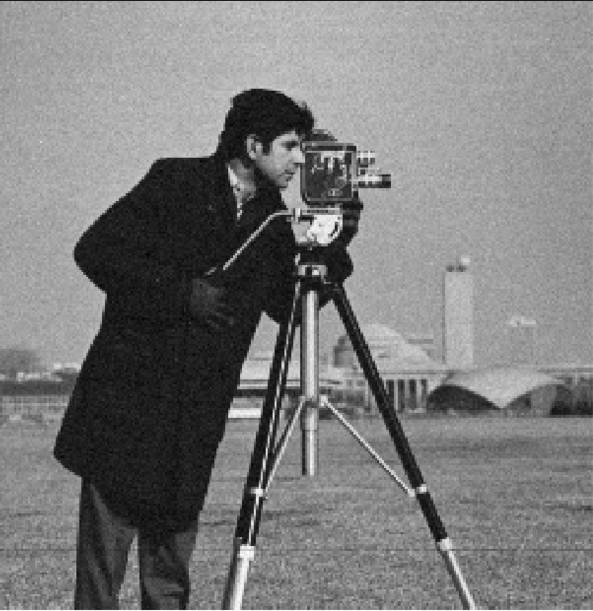
\includegraphics[scale=0.5]{noisyCameraman.png} % scale 75%
\end{figure}
    \begin{figure}[H]
	\centering
	\caption{Manipulated Image }
	\label{fig:Graphic}
	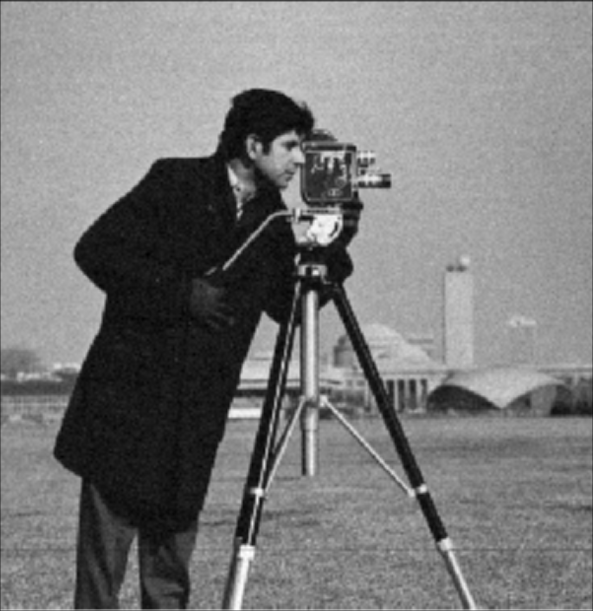
\includegraphics[scale=0.3]{last.png} % scale 75%
\end{figure}
\end{document}

 
